%!TEX root = ../../dokumentation.tex

\section{Service-Layer}
Der Service-Layer besteht aus einem Node-Red Server, der in einem Docker-Container läuft. Das hat den Vorteil, dass die Anwendung beliebig umgezogen oder skaliert werden kann. Zusätzlich empfängt der Server die Daten aus dem \ac{TTN} über \ac{MQTT} und speichert sie lokal in der \emph{Kontext}-Variablen und persistent als \ac{JSON}-Dokument ab. Dadurch können die Daten auch nach einem Neustart der Anwendung weiter verwendet werden. Abbildung \ref{fig:node-red} zeigt die folgenden drei Prozesse in Node-Red:

\begin{itemize}
    \item \textbf{Initialisierung}: Der erste \emph{Flow}, der beim Serverstart einmalig ausgeführt wird. Er lädt das gespeicherte \ac{JSON}-Dokument und setzt die \emph{Kontext}-Variablen auf die gespeicherten Werte.
    \item \textbf{Verbindung zum \ac{TTN}-Server}: Dieser Prozess wird für jede im \ac{TTN} empfangene und weitergeleitete Nachricht ausgeführt und speichert die empfangenen \ac{GPS}- und Sensor-Informationen im \ac{JSON}-Dokument bzw. Kontext des Servers.
    \item \textbf{App Anfrage}: Für jede empfangene \ac{HTTP}-Anfrage an die Route \emph{server-adresse:1880/device-id} wird der \emph{Flow} ausgeführt. Er lädt die Daten für die mitgelieferte \emph{device-id} und schickt sie als Antwort zurück an die App.
\end{itemize}

\begin{figure}[!htbp]
    \centering
    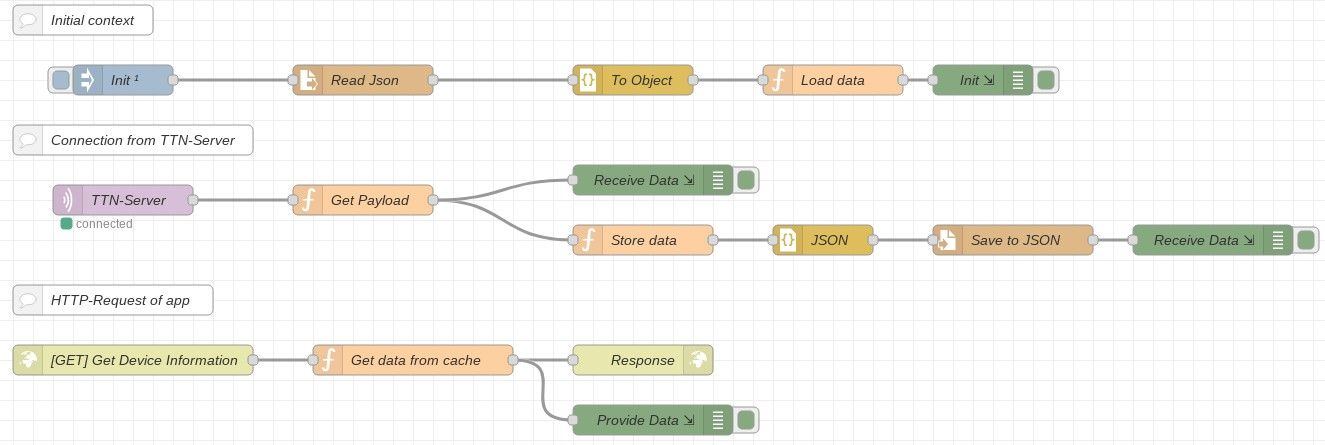
\includegraphics[width=1\linewidth]{images/node-red.jpg}
    \caption[Node-Red Serverarchitektur für das Smart-Lock]{Node-Red Serverarchitektur für das Smart-Lock}
    \label{fig:node-red}
\end{figure}

Außerdem wird der Server in der Azure-Cloud, auf einem Ubuntu-Server gehostet. Dadurch ist der Server aus dem Internet zugänglich und die Daten können jederzeit vom Benutzer abgerufen werden.

Zusammengefasst, deckt der Server, den Service-Layer mit persistenter Speicherung ab, indem er Nachrichten aus dem Network-Layer empfängt und an das Application-Layer weiterleitet. Zusätzlich werden die Daten im Server gespeichert, um sie jederzeit abfragen zu können, auch wenn der Server neu gestartet wurde. In Zukunft lässt sich das System weiter skalieren oder auf einem eigenen Server hosten, da es in einem Docker-Container läuft.